\documentclass[11pt,a4paper]{article}

\usepackage[margin=2cm]{geometry}
\usepackage[T1]{fontenc}
\usepackage{lmodern}
\usepackage{microtype}
\usepackage{amsmath}
\usepackage{graphicx}
\usepackage{booktabs}
\usepackage{tabularx}
\usepackage{array}
\usepackage{xcolor}
\usepackage{enumitem}
\usepackage{caption}
\usepackage{subcaption}
\usepackage{titlesec}
\usepackage[hidelinks]{hyperref}

\graphicspath{{figures/}}
\definecolor{accent}{RGB}{0,120,170}
\titleformat{\section}{\large\bfseries\color{accent}}{\thesection}{0.6em}{}
\titleformat{\subsection}{\normalsize\bfseries}{\thesubsection}{0.5em}{}
\titlespacing*{\section}{0pt}{1.0ex plus 0.4ex}{0.6ex}
\titlespacing*{\subsection}{0pt}{0.8ex plus 0.3ex}{0.4ex}
\captionsetup{font=small,labelfont=bf,skip=3pt}
\captionsetup[sub]{font=footnotesize}
\setlist{nosep,leftmargin=*}
\setlength{\parskip}{0.45ex}
\setlength{\parindent}{0pt}
\newcolumntype{L}{>{\raggedright\arraybackslash}X}

\begin{document}

% ------------------------------------------------------------------ cover page
\begin{titlepage}
  \centering
  \vspace*{1.2cm}
  {\large Introduction to Augmented Reality and Virtual Reality (AIL7110)\par}
  \vspace{0.3cm}
  {\large Assignment 02\par}
  \vspace{1.6cm}
  {\color{accent}\rule{\textwidth}{1.2pt}\par}
  \vspace{0.5cm}
  {\Huge\bfseries WorldForge Robotics Lab\par}
  \vspace{0.35cm}
  {\Large Development of a Virtual Environment Using Unity\par}
  \vspace{0.4cm}
  {\color{accent}\rule{\textwidth}{1.2pt}\par}
  \vspace{1.2cm}
  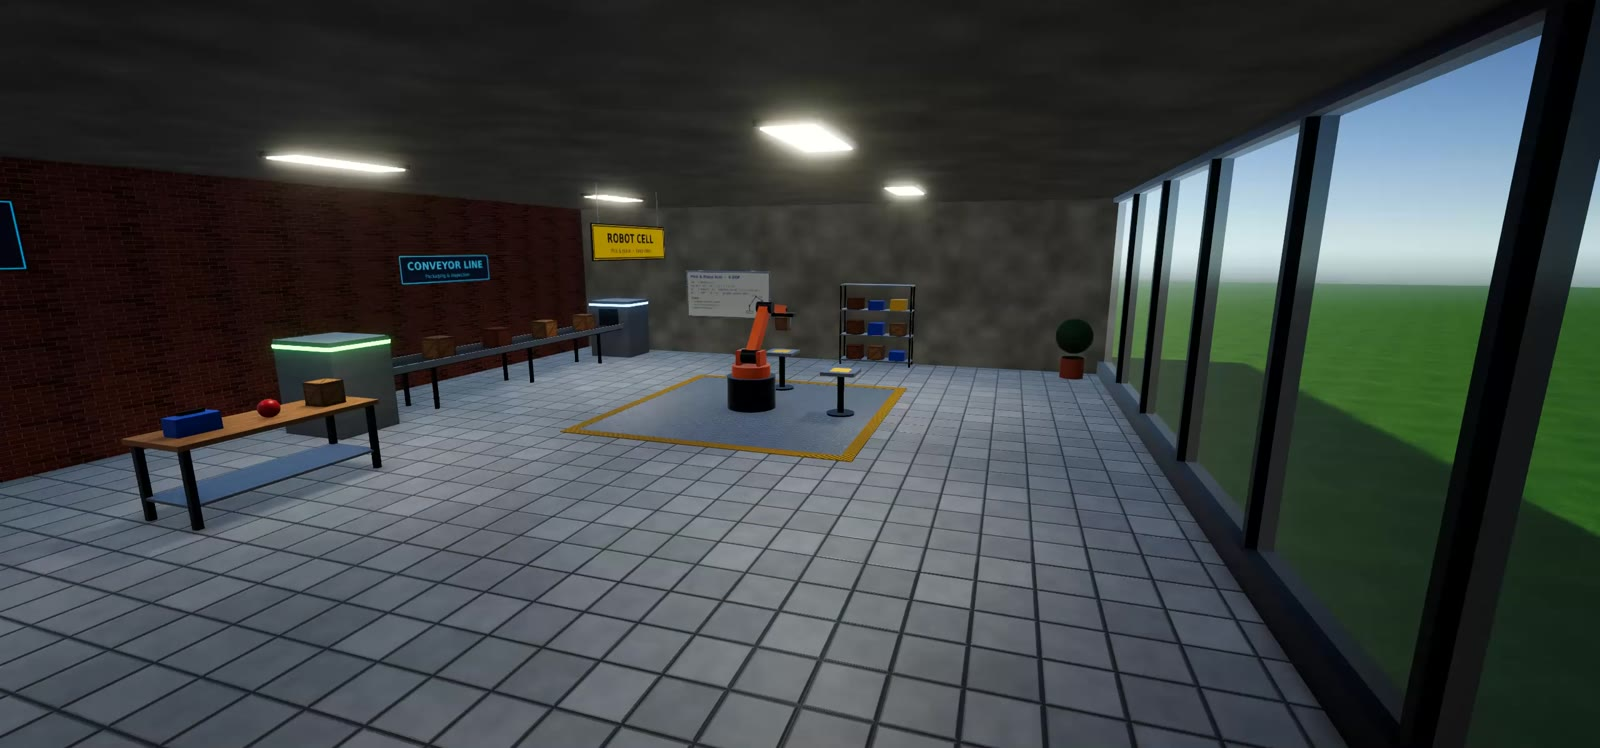
\includegraphics[width=\textwidth]{overview.jpg}\par
  \vspace{1.6cm}
  {\large
  \begin{tabular}{rl}
    \textbf{Name:} & Sahil Narkhede \\[2pt]
    \textbf{Roll No.:} & B23CS1060 \\[2pt]
    \textbf{Course:} & AIL7110 -- Introduction to Augmented Reality and Virtual Reality \\[2pt]
    \textbf{Engine:} & Unity 6.3 LTS (Universal Render Pipeline) \\
  \end{tabular}\par}
  \vfill
  {\large 23 October 2026\par}
\end{titlepage}

% ------------------------------------------------------------------ 1
\section{Objective and Environment Overview}

The objective of this assignment was to build a 3D virtual environment in Unity and use it to practise the
basic concepts of virtual world creation: modelling and placing objects, designing materials and lighting,
navigating with a camera, and interacting with the scene.

I built \textbf{WorldForge Robotics Lab}, a single-room robotics laboratory that the user explores in first
person. The room is $20\,\text{m} \times 14\,\text{m}$ with a 4\,m ceiling. It has a red-brick back wall, concrete
side walls and a continuous glass wall on the north side, which looks out over open green ground under a
daylight sky. The room is organised into five zones:

\begin{itemize}
  \item \textbf{Robot cell} (centre-left): an orange 4-axis robot arm on a pedestal, standing on a diamond-plate
        floor marked with yellow-and-black hazard stripes, with two small tables it moves a crate between.
  \item \textbf{Conveyor line} (along the brick wall): an 8\,m belt that carries wooden crates between an input
        and an output housing.
  \item \textbf{Workstations} (east wall): two desks with monitors showing a code editor and a telemetry dashboard.
  \item \textbf{Workbench} (centre): a wooden bench holding a crate, a rubber ball and a toolbox the user can pick up.
  \item \textbf{Storage} (west wall): a metal shelf with boxes and bins, and a whiteboard showing the robot arm's equations.
\end{itemize}

% ------------------------------------------------------------------ 2
\section{3D Objects: Creation and Placement}

All objects were built inside Unity from primitive shapes (cubes, cylinders, spheres and quads), scaled and
combined into larger objects. No external 3D models were imported. Every object is built at real-world scale
(a desk is 0.75\,m high and the eye height is 1.62\,m), so the space reads correctly in first person.
The final scene contains about 200 objects, 162 of which are rendered meshes.

\begin{table}[h]
\centering\small
\begin{tabularx}{\textwidth}{@{}p{3.1cm}Lp{3.3cm}@{}}
\toprule
\textbf{Object} & \textbf{How it is built} & \textbf{Placement} \\
\midrule
Room shell & Floor, ceiling, roof and three solid walls; the glass wall is a curb, 7 metal mullions, 8 glass panes and a top beam & Encloses the whole lab \\
Robot arm & Pedestal, rotating base, upper arm, forearm, wrist and two-finger gripper, each part attached to the previous joint & Centre of the robot cell \\
Pick/place tables & Steel top, column and foot with a yellow target mark & Two sides of the robot cell \\
Conveyor & Belt, side rails, legs, two end housings with light strips, five crates & Along the brick wall \\
Workstations ($\times$2) & Desk, monitor with screen, keyboard and chair & East wall \\
Workbench & Top, legs and lower shelf, with a crate, ball and toolbox on top & Centre of the room \\
Shelf & Four uprights, four boards and nine boxes and bins & West wall \\
Details & Ceiling light panels, whiteboard, three signs, two potted plants, light switch & Walls and corners \\
Outside & Large flat grass ground plane & Around the building \\
\bottomrule
\end{tabularx}
\caption{Main 3D objects in the environment.}
\end{table}

% ------------------------------------------------------------------ 3
\section{Environment Design: Materials, Colours, Textures and Lighting}

\textbf{Materials and colours.} The project uses the Universal Render Pipeline (URP) with physically based
\emph{Lit} materials, so each surface has its own colour, metalness and smoothness. Steel parts are metallic
and glossy; wood, fabric and concrete are matte. The palette is deliberately simple: neutral greys for the
room, safety orange for the robot, yellow and black for hazard markings, and cyan accents on the signs and
light strips. In total there are 46 materials.

\textbf{Textures.} I generated 12 tileable surface textures (floor tiles, concrete, brick, wood grain,
brushed metal, diamond tread plate, hazard stripes, rubber belt, wooden crates, fabric, grass and leaves).
Nine of them also have a matching normal map, which adds surface relief such as tile grout and brick mortar. Each texture is tiled to match the real size of the
surface it covers. A further six text textures (the signs, the whiteboard and the two monitor screens) were
drawn with Python and Pillow. The glass panes are transparent and highly smooth, and they do not cast
shadows, so daylight reaches the interior.

\textbf{Lighting.} A directional sun with soft shadows and a procedural sky light the scene, together with
three-colour ambient light (sky, horizon and ground). Inside, six ceiling spot lights with soft shadows sit
under glowing light panels. A reflection probe gives the metal surfaces realistic reflections, and light fog
softens the horizon outside. Post-processing adds ACES tone mapping, bloom on bright surfaces, slight
contrast and saturation adjustment, a vignette, ambient occlusion and anti-aliasing.

\begin{figure}[h]
  \centering
  \begin{subfigure}{0.49\textwidth}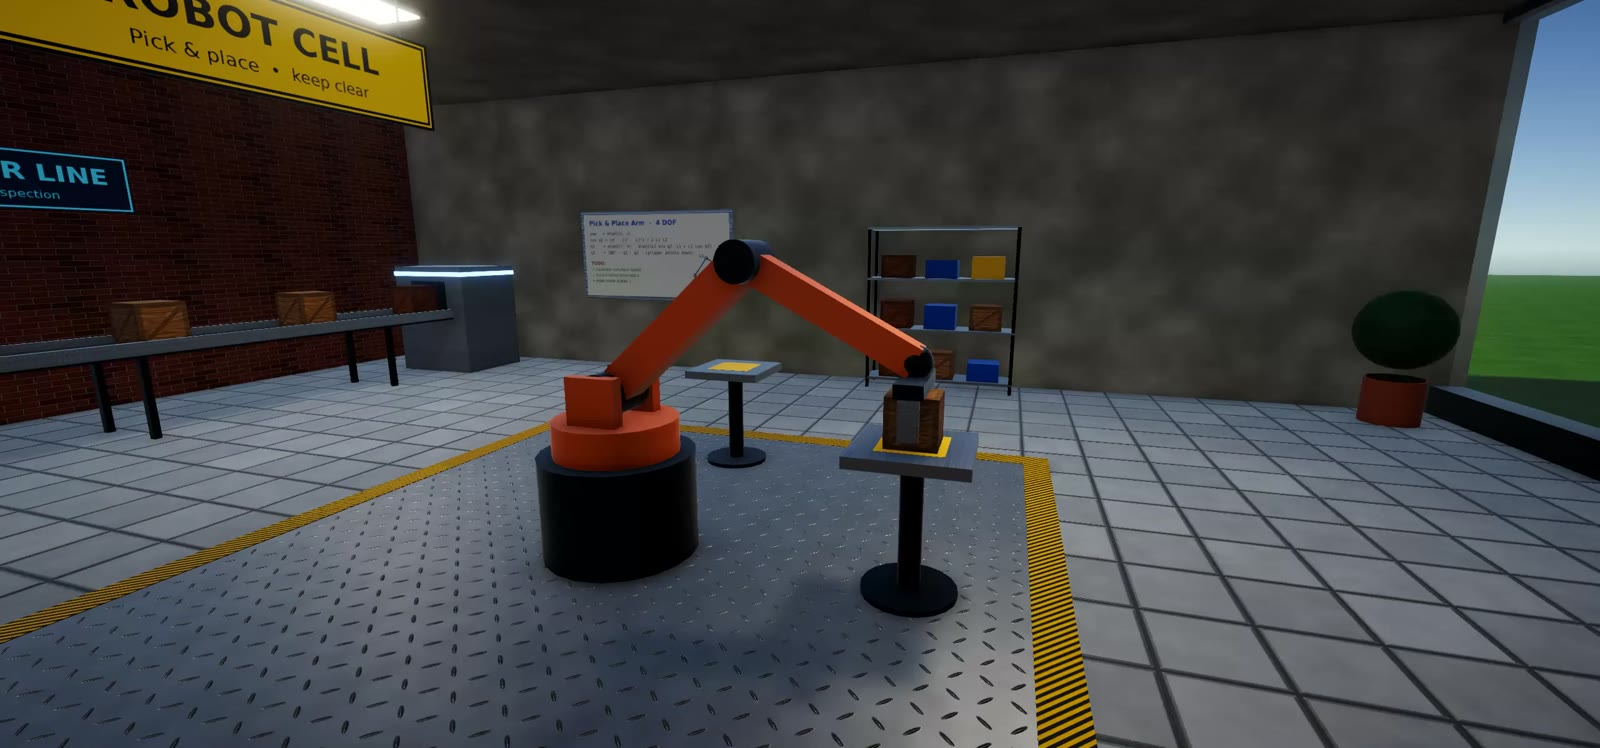
\includegraphics[width=\linewidth]{robot_cell.jpg}\caption{Robot cell: the arm gripping a crate}\end{subfigure}\hfill
  \begin{subfigure}{0.49\textwidth}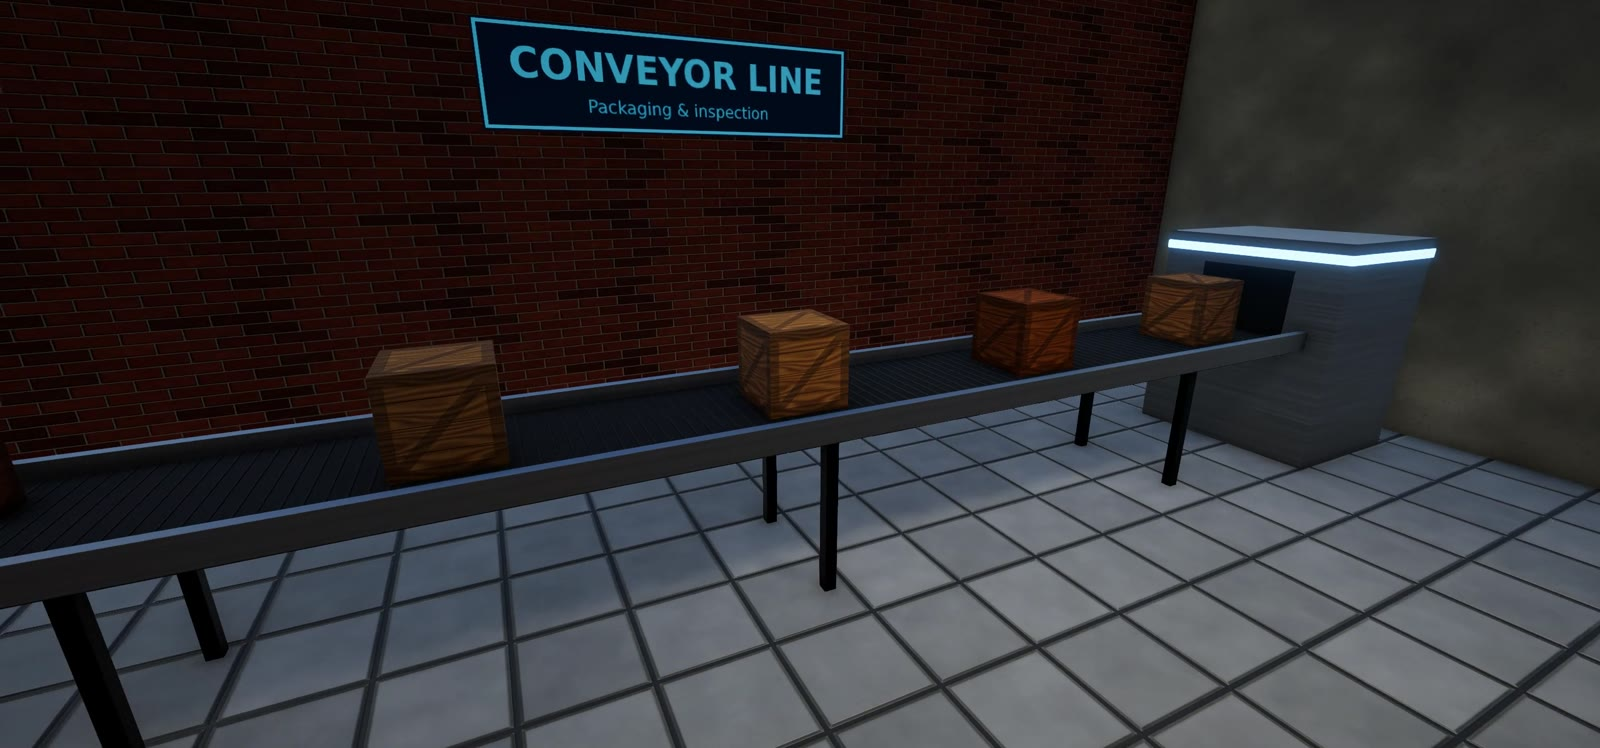
\includegraphics[width=\linewidth]{conveyor.jpg}\caption{Conveyor line along the brick wall}\end{subfigure}\\[4pt]
  \begin{subfigure}{0.49\textwidth}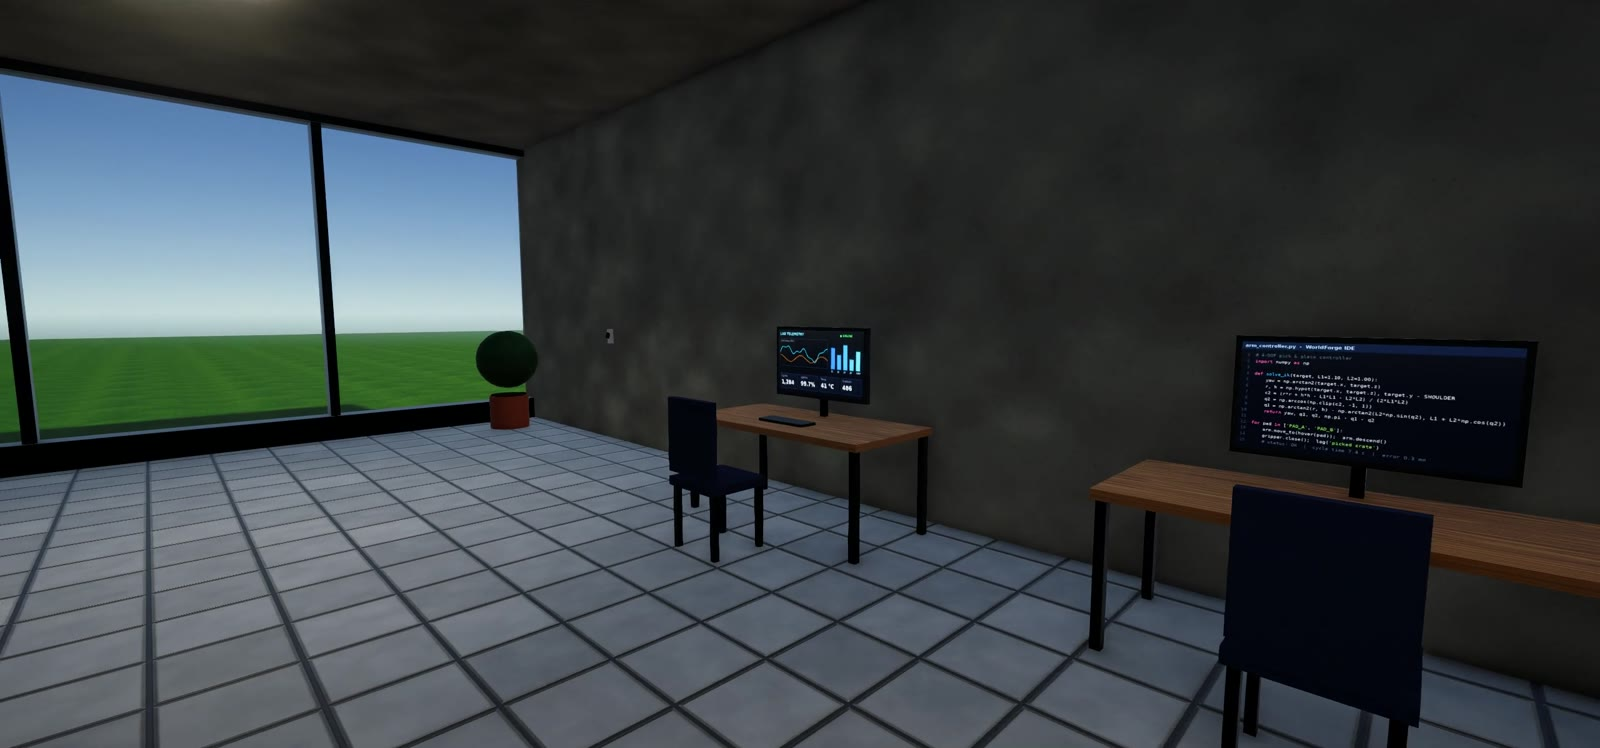
\includegraphics[width=\linewidth]{workstations.jpg}\caption{Workstations with monitors and chairs}\end{subfigure}\hfill
  \begin{subfigure}{0.49\textwidth}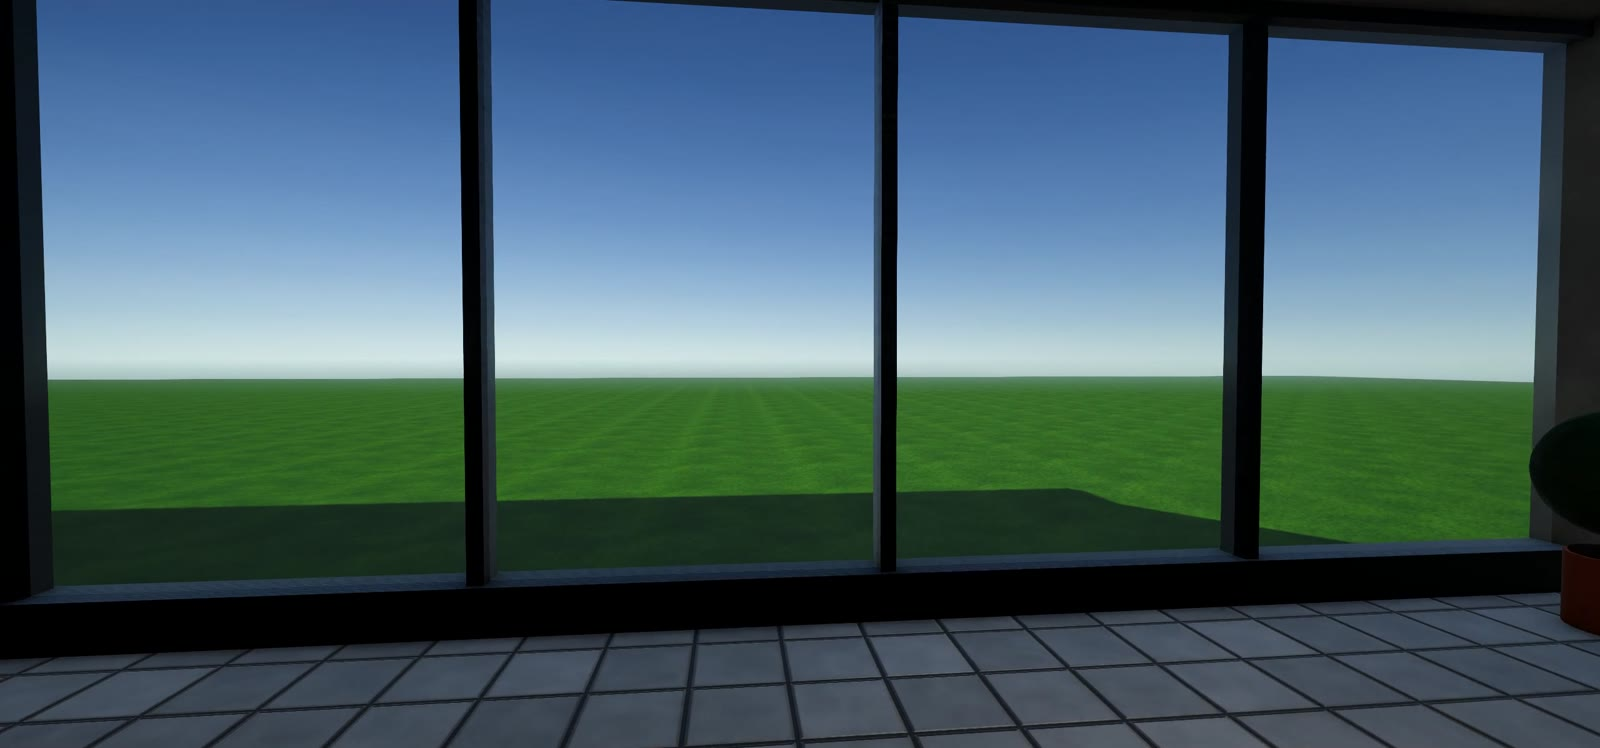
\includegraphics[width=\linewidth]{window_view.jpg}\caption{Glass wall overlooking the green ground}\end{subfigure}
  \caption{Zones of the lab, showing the materials, textures and lighting.}
\end{figure}

% ------------------------------------------------------------------ 4
\section{Camera Setup and Navigation}

The user explores the lab with a \textbf{first-person camera} attached to a character controller (a capsule
1.8\,m tall, 70$^\circ$ field of view). The character walks at 3.2\,m/s, sprints at 6\,m/s, can jump, and is
affected by gravity. Walls, glass panes and furniture all have colliders, so the user cannot walk through them.
Mouse look is lightly smoothed and the vertical angle is limited to $\pm$80$^\circ$. Pressing \textbf{V}
switches to a \textbf{third-person camera} behind a simple avatar. This camera moves closer when a wall gets in
the way, so it never clips through geometry. Pressing \textbf{T} starts a \textbf{guided tour}: the camera glides
along a smooth path through eight viewpoints with cinematic black bars. This tour was used to record the
submission video. An on-screen display shows the lab name, the current camera mode, a crosshair and a controls
panel.

\begin{table}[h]
\centering\small
\begin{tabular}{@{}ll@{\hspace{2.2em}}ll@{}}
\toprule
\textbf{Key} & \textbf{Action} & \textbf{Key} & \textbf{Action} \\
\midrule
W A S D / arrows & Move & E / left click & Interact, pick up, drop \\
Mouse & Look around & Right click & Throw held object \\
Shift & Sprint & R (hold) & Rotate held object \\
Space & Jump & V & First / third person \\
T & Guided camera tour & H / U & Hide help / hide all UI \\
\bottomrule
\end{tabular}
\caption{Navigation and interaction controls.}
\end{table}

% ------------------------------------------------------------------ 5
\section{Interaction}

When the user aims at an interactive object, the object brightens slightly and a label below the crosshair
names it and shows the available action. Pressing \textbf{E} or clicking performs that action:

\begin{itemize}
  \item \textbf{Robot arm:} runs a full pick-and-place cycle. The arm moves above the crate, lowers, closes its
        gripper, lifts the crate, turns and places it on the other table, then returns home. Its joint angles are
        calculated in real time so the gripper always reaches the target, and a status lamp on the pedestal shows
        whether the arm is busy.
  \item \textbf{Conveyor belt:} stops or starts the line. The crates move along the belt while its surface scrolls.
  \item \textbf{Light switch:} turns the six ceiling lights and their glowing panels on or off.
  \item \textbf{Workbench items:} the crate, ball and toolbox are physics objects. The user can pick them up,
        carry and rotate them, drop them or throw them; they then fall, bounce and collide realistically.
\end{itemize}

\begin{figure}[h]
  \centering
  \begin{subfigure}{0.325\textwidth}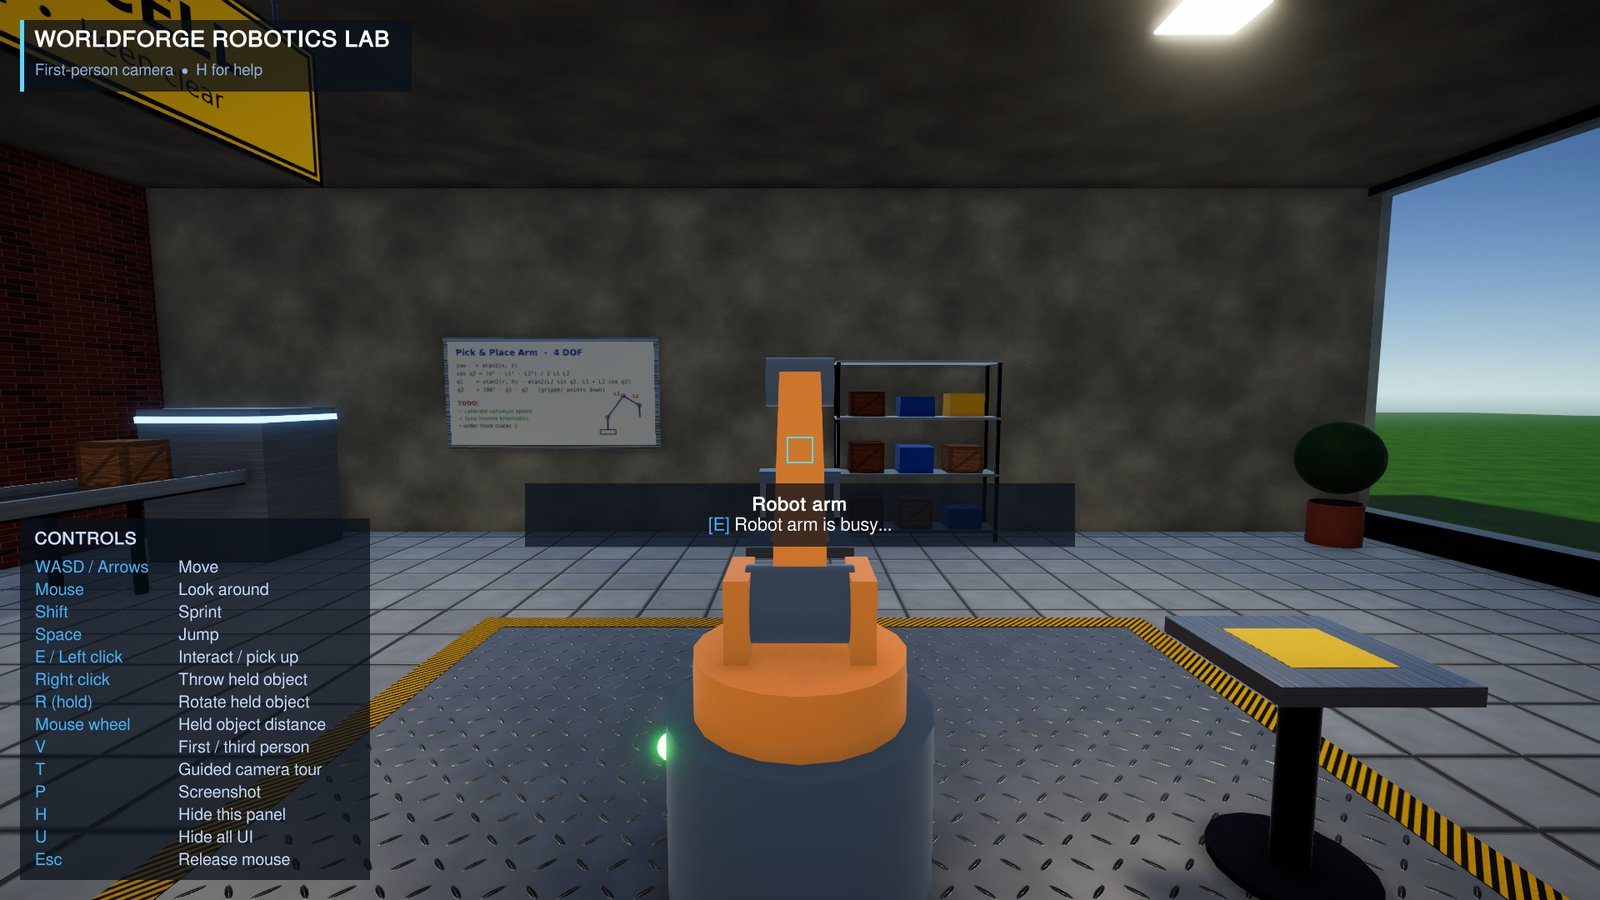
\includegraphics[width=\linewidth]{hud_interact.jpg}\caption{Aiming at the robot arm}\end{subfigure}\hfill
  \begin{subfigure}{0.325\textwidth}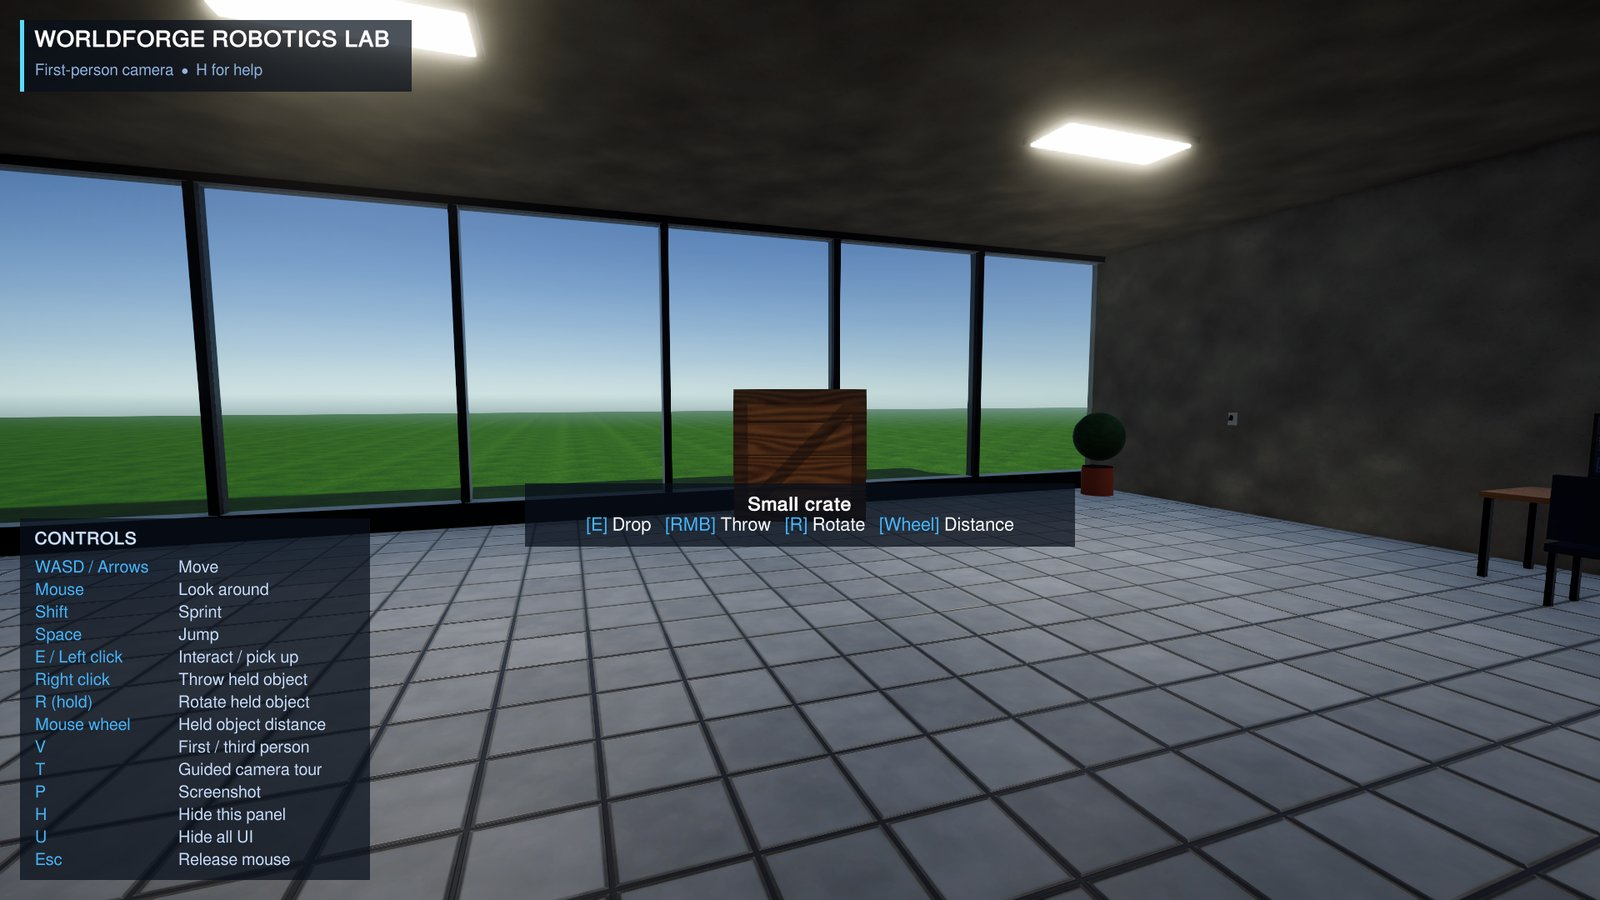
\includegraphics[width=\linewidth]{hud_holding.jpg}\caption{Carrying a crate}\end{subfigure}\hfill
  \begin{subfigure}{0.325\textwidth}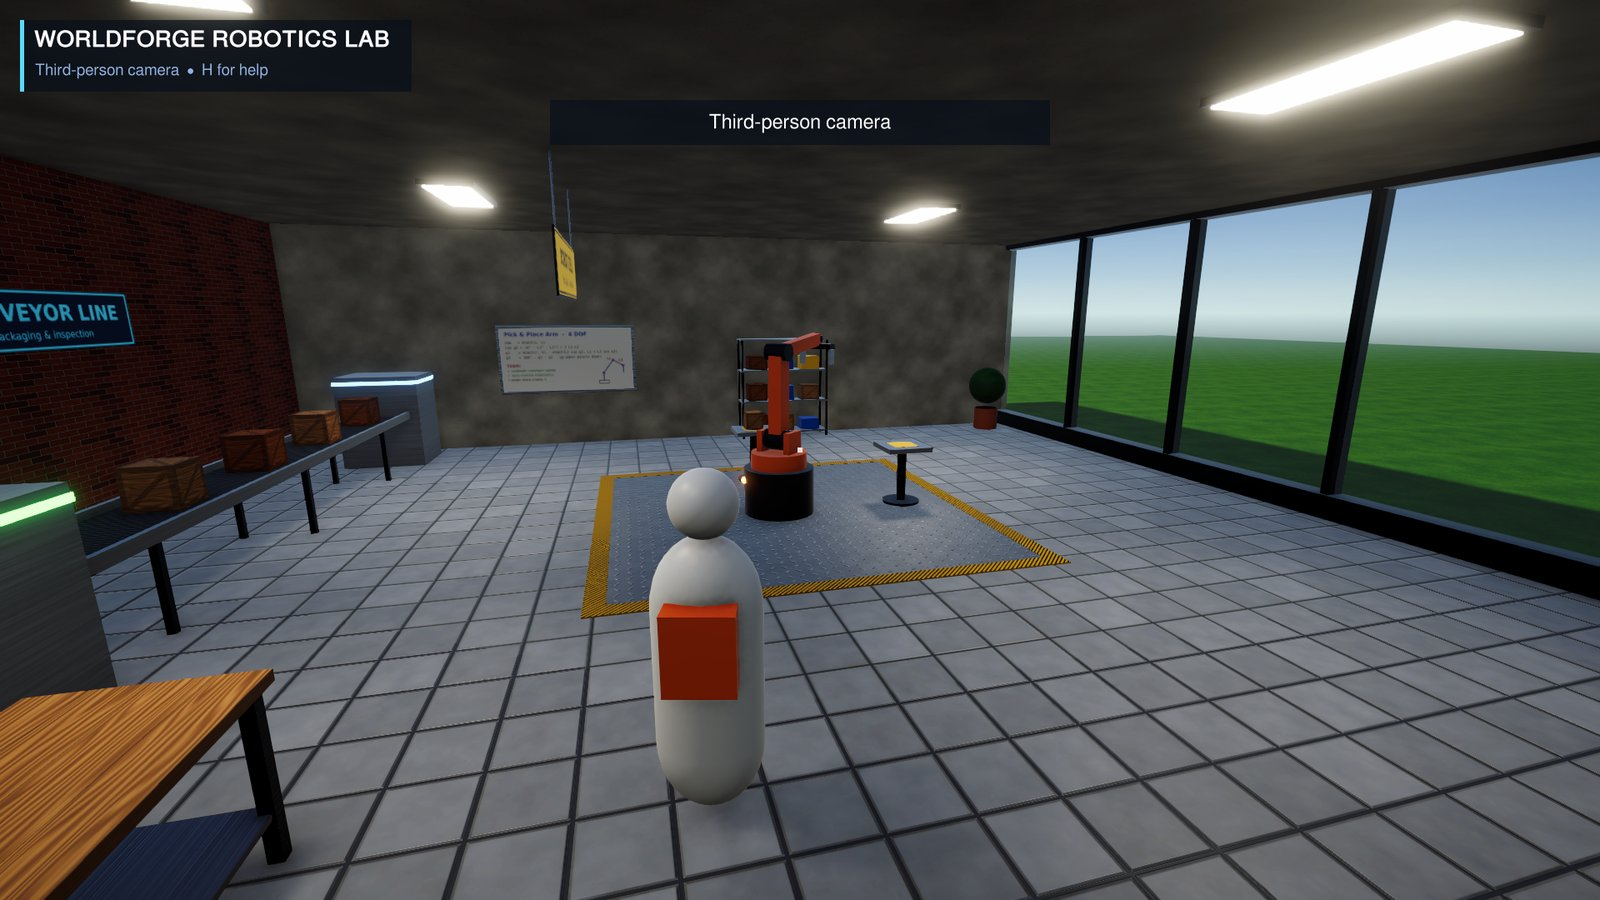
\includegraphics[width=\linewidth]{hud_third_person.jpg}\caption{Third-person camera}\end{subfigure}
  \caption{Interaction prompts, carrying an object, and the third-person view.}
\end{figure}

% ------------------------------------------------------------------ 6
\section{Tools Used}

\begin{table}[h]
\centering\small
\begin{tabularx}{\textwidth}{@{}p{6.2cm}L@{}}
\toprule
\textbf{Tool} & \textbf{Purpose} \\
\midrule
Unity 6.3 LTS (6000.3.26f1), Unity Hub & Game engine and editor used to build, test and run the environment \\
Universal Render Pipeline 17.3 & Physically based materials, real-time lighting, shadows and post-processing \\
Unity Input System 1.20 & Keyboard and mouse input for navigation and interaction \\
Unity Recorder 5.1.7 & Recording the guided tour at 2560$\times$1440, 60\,fps \\
C\# & Scripts for movement, cameras, interactions and the guided tour \\
Python 3 with Pillow & Drawing the sign, whiteboard and monitor-screen textures \\
FFmpeg & Converting the recorded video to H.264 MP4 \\
Git and GitHub, Ubuntu 24.04 & Version control; development operating system \\
\bottomrule
\end{tabularx}
\caption{Software used.}
\end{table}

% ------------------------------------------------------------------ 7
\section{Development Process}

\begin{enumerate}
  \item \textbf{Planning.} I chose the robotics-lab theme, sketched a floor plan with five zones, and mapped
        each assignment requirement to concrete features.
  \item \textbf{Project setup.} I created a Unity 6 project from the URP 3D template and configured the input
        system, quality settings and post-processing.
  \item \textbf{Textures and materials.} I created the tileable surface textures and the text textures, then
        set up a material for each surface type with suitable colour, metalness and smoothness.
  \item \textbf{Scene assembly.} I built the room shell first, then each zone from primitives at real-world
        scale. The robot arm was built as a chain of joints so each part moves with the one before it.
        The whole scene can be regenerated from the editor so it stays consistent.
  \item \textbf{Lighting.} I added the sun, sky, ceiling lights, reflection probe and post-processing, then
        refined them by comparing screenshots. For example, I brightened the dark ceiling and toned down the
        object highlight.
  \item \textbf{Navigation and interaction.} I added the first- and third-person controller, the
        interaction system, the robot arm's pick-and-place behaviour, the conveyor, the light switch, the
        objects that can be picked up, and the guided tour.
  \item \textbf{Testing.} I play-tested in the editor and ran an automated check on a standalone build. The check
        confirmed the robot cycle, conveyor movement, light switching, walking, wall collisions, picking up and
        dropping objects, and the tour, and all checks passed.
  \item \textbf{Simplification.} An earlier version also had an outdoor garden, a door and day/night cycling.
        For the submission I reduced the scope to a focused, polished lab with the glass wall and green ground.
  \item \textbf{Recording.} I recorded the guided tour with Unity Recorder at QHD (2560$\times$1440, 60\,fps)
        and converted it to MP4.
\end{enumerate}

% ------------------------------------------------------------------ 8
\section{Submission Contents}

\begin{itemize}
  \item \textbf{Video:} \texttt{WorldForge\_v2\_Tour\_1440p.mp4}, a guided walkthrough of the lab
        (2560$\times$1440, 60\,fps, H.264).
  \item \textbf{Unity project:} the \texttt{worldforge-v2} folder (\texttt{Assets}, \texttt{Packages},
        \texttt{ProjectSettings}). To run it, open the folder in Unity Hub with Unity 6.3, let the
        \texttt{WorldForge} scene open, and press \textbf{Play}. To re-record the tour, choose
        \textbf{WorldForge $\rightarrow$ Record Guided Tour (QHD)}.
  \item \textbf{Report:} this document.
\end{itemize}

The finished environment meets every requirement of the assignment: more than five 3D objects placed at
real-world scale, textured materials with realistic lighting, first- and third-person navigation, and several
working interactions.

\end{document}
